%% This is file `elsarticle-template-1-num.tex',
%%
%% Copyright 2009 Elsevier Ltd
%%
%% This file is part of the 'Elsarticle Bundle'.
%% ---------------------------------------------
%%
%% It may be distributed under the conditions of the LaTeX Project Public
%% License, either version 1.2 of this license or (at your option) any
%% later version.  The latest version of this license is in
%%    http://www.latex-project.org/lppl.txt
%% and version 1.2 or later is part of all distributions of LaTeX
%% version 1999/12/01 or later.
%%
%% Template article for Elsevier's document class `elsarticle'
%% with numbered style bibliographic references
%%
%% $Id: elsarticle-template-1-num.tex 149 2009-10-08 05:01:15Z rishi $
%% $URL: http://lenova.river-valley.com/svn/elsbst/trunk/elsarticle-template-1-num.tex $
%%
\documentclass[preprint,5p, twocolumn, authoryear]{elsarticle}

%% Use the option review to obtain double line spacing
%% \documentclass[preprint,review,12pt]{elsarticle}

%% Use the options 1p,twocolumn; 3p; 3p,twocolumn; 5p; or 5p,twocolumn
%% for a journal layout:
%% \documentclass[final,1p,times]{elsarticle}
%% \documentclass[final,1p,times,twocolumn]{elsarticle}
%% \documentclass[final,3p,times]{elsarticle}
%% \documentclass[final,3p,times,twocolumn]{elsarticle}
%% \documentclass[final,5p,times]{elsarticle}
%% \documentclass[final,5p,times,twocolumn]{elsarticle}

%% The graphicx package provides the includegraphics command.
\usepackage{graphicx}
%% The amssymb package provides various useful mathematical symbols
\usepackage{amsmath}   % Extra math commands and environments from the AMS
\usepackage{amssymb}   % Special symbols from the AMS
\usepackage{amsthm}    % Enhanced theorem and proof environments from the AMS
\usepackage{latexsym}  % A few extra LaTeX symbols
\usepackage{array}
\usepackage{makecell}
\usepackage{units}
\usepackage{xcolor}
%% The lineno packages adds line numbers. Start line numbering with
%% \begin{linenumbers}, end it with \end{linenumbers}. Or switch it on
%% for the whole article with \linenumbers after \end{frontmatter}.
\usepackage{lineno}
\usepackage[singlelinecheck=false]{caption}

%\biboptions{longnamesfirst, semicolon}
%% natbib.sty is loaded by default. However, natbib options can be
%% provided with \biboptions{...} command. Following options are
%% valid:

%%   round  -  round parentheses are used (default)
%%   square -  square brackets are used   [option]
%%   curly  -  curly braces are used      {option}
%%   angle  -  angle brackets are used    <option>
%%   semicolon  -  multiple citations separated by semi-colon
%%   colon  - same as semicolon, an earlier confusion
%%   comma  -  separated by comma
%%   numbers-  selects numerical citations
%%   super  -  numerical citations as superscripts
%%   sort   -  sorts multiple citations according to order in ref. list
%%   sort&compress   -  like sort, but also compresses numerical citations
%%   compress - compresses without sorting
%%
%% \biboptions{comma,round}

% \biboptions{}
\newcommand{\useq}{\mathbf{u}}
\newcommand{\xseq}{\mathbf{x}}
\newcommand{\bbR}{\mathbb{R}}
\newcommand{\bbW}{\mathbb{W}}
\newcommand{\bbU}{\mathbb{U}}
\newcommand{\bbI}{\mathbb{I}}
\newcommand{\bbX}{\mathbb{X}}
\newcommand{\bbP}{\mathbb{P}}

\graphicspath{{./}{./figures/}{./figures/paper/}}

\newdefinition{assumption}{Assumption}
\newdefinition{prop}{Proposition}
\newdefinition{definition}{Definition}
\newdefinition{rmk}{Remark}
\newtheorem{thm}{Theorem}

\journal{Elsevier}

\begin{document}

\begin{frontmatter}

%% Title, authors and addresses

\title{Industrial, large-scale model predictive control 
with structured neural networks}

%% use the tnoteref command within \title for footnotes;
%% use the tnotetext command for the associated footnote;
%% use the fnref command within \author or \address for footnotes;
%% use the fntext command for the associated footnote;
%% use the corref command within \author for corresponding author footnotes;
%% use the cortext command for the associated footnote;
%% use the ead command for the email address,
%% and the form \ead[url] for the home page:
%%
%% \title{Title\tnoteref{label1}}
%% \tnotetext[label1]{}
\author[label1]{Pratyush Kumar\corref{cor1}}
\ead{pratyushkumar@ucsb.edu}
%% \ead[url]{home page}
%% \fntext[label2]{}
\cortext[cor1]{Corresponding Author}
%% \fntext[label3]{}

\author[label1]{James B. Rawlings}
\ead{jbraw@ucsb.edu}

\author[label2]{Stephen J. Wright}
\ead{swright@cs.wisc.edu}

\address[label1]{Department of Chemical Engineering, University of California, Santa Barbara, CA 93106, United States}
\address[label2]{Computer Sciences Department, University of Wisconsin-Madison, Madison, WI 53706, United States}

\begin{abstract}
The design of neural networks (NNs) is presented 
for treating large, linear model predictive control (MPC) applications that 
are out of reach with available quadratic programming (QP)
solvers. First, we introduce a new feedforward
network architecture that enables practitioners to 
obtain offset-free closed-loop performance with NNs.
Second, we discuss the data generation procedure 
to sample the relevant state space for the network 
training based on anticipated online setpoint changes and
plant disturbances. Third, we use the 
input-to-state stability results 
available in the MPC literature
and establish robustness 
properties of NN controllers.
Finally, we present illustrative
simulation studies on 
process control examples. 
We apply the NN design approach
and compare the performance with online QP based MPC on an industrial crude
distillation unit model with 252 states, 32 control inputs, 
and a control-sample horizon length of 140. Parallel computing 
is used for data generation and graphical processing units are used for
network training. All the anticipated plant operational scenarios 
with setpoints and disturbances that may change
during operation must be sampled for NN training.
After the offline design phase, 
NNs execute MPC 
three to five orders of magnitude faster
than an available QP solver with less than $1\%$
loss in the closed-loop performance.
\end{abstract}

\begin{keyword}
Model predictive control \sep machine learning \sep 
deep neural networks \sep large-scale problems
\end{keyword}

\end{frontmatter}

%% main text
\section{Introduction} \label{sec:introduction}

Model predictive control (MPC) is an online 
optimization based feedback control technology. A dynamic model 
of the plant is used to make forecasts of the plant measurements
in response to the actuator movements, and an optimization
is solved in real time to determine the optimal actuator
move to be applied to the plant. For linear plant models, 
the optimization to be solved online is a quadratic program (QP).
The development 
of efficient QP algorithms 
\citep*{kouzoupis:frison:zanelli:diehl:2018, wright:2019}
allowed practitioners to adopt MPC
in process industries \citep*{qin:badgwell:2003, lahiri:2017}.

An alternative strategy to 
real time optimization for the deployment of MPC 
is to characterize the MPC feedback law
as a piecewise affine function defined on 
polyhedral partitions of the state space, 
and use the feedback law online
\citep*{bemporad:morari:dua:pistikopoulos:2002, 
seron:goodwin:dedona:2003}.
The real time computation in this approach is 
reduced to a table look-up in the state space
based on the current value of parameters 
in the QP such as the state estimate and some 
steady-state targets that are computed for 
offset-free control. The number of polyhedral 
partitions of the state space grows exponentially
with model dimensions, however. Thereby prohibiting 
the deployment of this strategy on large-scale 
systems.

The MPC feedback law can be approximated using 
parametric functions such as polynomials
\citep*{kvasnica:lofberg:fikar:2011}, 
various types of piecewise affine functions
\citep*{bemporad:oliveri:poggi:storace:2011, wen:ma:ydstie:2009},
and neural networks (NNs) \citep*{cavagnari:magni:scattolini:1999}.
Among the
function approximators, NNs that use the rectified linear unit 
(ReLU) as the activation function 
have gained attention recently 
\citep*{chen:saulnier:atanasov:lee:kumar:pappas:morari:2018, 
karg:lucia:2020, paulson:mesbah:2020, lovelett:dietrich:lee:kevrekidis:2020}
to approximate
the MPC feedback law due to their ability to represent complex 
piecewise affine functions
\citep*{montufar:pascanu:cho:bengio:2014}
and execute MPC faster in real time than QP solvers. 
The proposed NN design approach in 
these works is to generate training 
data for the NN by solving QPs offline
for a set of feasible states of the QP, use the
collected data to train a standard feedforward network, then 
use the trained NN as the feedback controller online.

To make progress in the size of control applications 
achievable with MPC, large problems
in which QP solvers fail to deliver the 
control in the available sample time should be addressed.
The scalability of the NN approach
to such problems with large model dimensions and 
control horizon length in the QP
has not been demonstrated. Two issues arise 
in these problems:
i) In a large dimensional state space,   
the entire set of feasible states of the QP cannot be sampled  
densely for the NN training. This issue is 
a form of the curse of dimensionality.
ii) One may sample the state space partially
to avoid this problem, but the time required for the 
data generation can still be impractical
due to the long time required to solve a QP 
for each sampled state. 
We demonstrate in this article by case studies that
this latter issue can be resolved for a large size 
of problems with parallel 
computing, and the former issue by sampling the 
state space for typical plant operational scenarios.
The following feature must be present in the large-scale
application of interest for the partial sampling scheme 
proposed in this article to be applicable:
for a particular operating mode of the plant, 
the number of frequently changing setpoints
and large magnitude disturbances 
must be reasonably small 
such that the entire large
dimensional state space is not visited during that
operation mode. 
The MPC feedback law 
can then be reliably approximated using NNs
for the different modes of plant operations driven by  
their respective set
of setpoint changes and disturbances.

From the above viewpoint, 
this article discusses the design of NNs
as an alternative to real time optimization in MPC, 
with an emphasis on large applications which 
are challenging with QP solvers. 
The focus of this article is on setpoint tracking 
MPC problems relevant for deployment in process industries.
We present a new feedforward network architecture to obtain
offset-free closed-loop performance with the NNs.
Additionally, we use the input-to-state
stability results \citep*{sontag:wang:1995}
available in the MPC literature, and establish
conditions under which the NN controller 
is robust to state estimation errors and process 
disturbances. We present case studies 
on process control examples which
demonstrate the scalability of the proposed NN design 
approach.

The related work by \cite*{chen:wang:atanasov:kumar:morari:2019}
demonstrates the scalability of NNs 
to approximate the MPC feedback law on systems with 
state dimensions upto thirty-six. The setpoint 
tracking offset-free MPC problem and state 
dimensions upto two-fifty considered in this 
article is not addressed in that work. 
\cite*{drgona:picard:kvasnica:helsen:2018}
takes a different approach for the scalability
of NN controllers, in which 
the dimensionality of the parameters in the MPC QP is first 
reduced using principal component analysis, and the 
NN controller is developed in a low dimensional state space.

The rest of this article is organized as follows. 
In the next section, we briefly review 
offset-free linear MPC. 
In Section \ref{sec:controller_design},
we discuss the NN 
controller design procedure.
We present the robustness property
of NNs in Section \ref{sec:robustness}.
Then, we present simulation studies
on two large process control examples
in Section \ref{sec:simulation_studies}
and conclude at the end of this article.

Notation. The symbols $\bbI$ and $\bbR$ are 
used to denote integers and reals respectively. 
Subscripts denote restrictions 
(e.g., $\bbR_{\geq 0}$ for nonnegative reals and 
$\bbI_{a:b}$ for integers in the 
closed interval $[a, b]$). The Euclidean norm 
is denoted by $\vert \cdot \vert$. A function 
$\alpha : \bbR_{\geq 0} \rightarrow \bbR_{\geq 0}$
is of class $\mathcal{K}$ if it is continuous, zero 
at zero, and strictly increasing. This function is of class 
$\mathcal{K}_{\infty}$ if it is of class $\mathcal{K}$
and unbounded ($\alpha(s) \rightarrow \infty$ as 
$s \rightarrow \infty$). A function
$\beta : \bbR_{\geq 0} \times \bbI_{\geq 0} \rightarrow \bbR_{\geq 0}$
is of class $\mathcal{K} \mathcal{L}$ if it is continuous,
for a fixed $k \in \bbI_{\geq 0}$, $\beta(\cdot, k)$ is of class $\mathcal{K}$,
and for a fixed $s \geq 0$, $\beta(s, \cdot)$ is nonincreasing
and satisfies $\textnormal{lim}_{k \rightarrow \infty} \beta(s, k) = 0$.
Given $V : X \rightarrow \bbR_{\geq 0}$ and $\tau > 0$, define 
$\textnormal{lev}_{\tau} V = \{ x \in X | V(x) \leq \tau \}$.
Bold symbols, e.g., $\mathbf{d}$ denote sequences, 
$d(k)$ denotes an element of $\mathbf{d}$ at time 
$k \in \bbI_{\geq 0}$, and $\mathbf{d}_i$ 
denotes the collection of elements of 
$\mathbf{d}$ for $k \in \bbI_{0:i-1}$.
Define $\vert \vert \mathbf{d}_i \vert \vert = 
\textnormal{max}_{k \in \bbI_{0:i-1}} \vert d(k) \vert$.
For a given vector $a$, lower and upper bounds 
($\underline{a}, \overline{a}$), define the saturation function 
as $\textnormal{sat}(a, \underline{a}, \overline{a}) = 
\{ a \ \textnormal{if} \ \underline{a} \leq a \leq \overline{a}; 
\underline{a} \ \textnormal{if} \ a < \underline{a};
\overline{a} \ \textnormal{if} \ \overline{a} < a \}$.

\section{Linear model predictive control} \label{sec:mpc}

\subsection{Model}
We consider a linear discrete time model augmented with an 
integrating disturbance model \citep{pannocchia:rawlings:2003}
\begin{align}\label{eq:ltimodel}
    x^+ = Ax + Bu + B_dd, \quad d^+ = d, \quad y = Cx + C_dd
\end{align}
in which $x \in \bbR^n$ is the state, 
$u \in \bbR^m$ is the control input, and
$d \in \bbR^d$ is the state of the disturbance
model. The matrices $A \in \bbR^{n \times n}$, 
$B \in \bbR^{n \times m}$,  
$C \in \bbR^{p \times n}$ denote the actuator to measurement 
model, and $B_d \in \bbR^{n \times d}$, $C_d \in \bbR^{p \times d}$
is the disturbance model.
The objective of the disturbance model
is to remove offset in the controlled 
plant measurements at steady
state operations and maintain
them at their setpoints.
We assume in the rest of this 
article that a Kalman filter can be constructed to 
estimate the model state ($\hat{x}$) and disturbance ($\hat{d}$) 
from measurements. 

\subsection{Target selector}
Given the disturbance estimate, the
input and controlled measurement setpoints,
we consider the following target selector QP
\begin{align}
    \min_{x_s, \ u_s}  \dfrac{1}{2} |u_{sp} - u_s|^2_{R_s}
\end{align}
subject to
\begin{align}  
    \begin{bmatrix}
        I -A & -B \\
        HC & 0
    \end{bmatrix} \begin{bmatrix}
        x_s \\
        u_s
    \end{bmatrix} &= \begin{bmatrix}
        B_d\hat{d} \\
        r_{sp} - HC_d\hat{d}
    \end{bmatrix} \\
    \underline{u} \leq u_s \leq \overline{u}
\end{align}
in which
($x_s, u_s$) is the 
target steady state pair,
$r=Hy$ are the controlled measurements
chosen as some subset 
or a linear combination of all the measurements,
($\underline{u}, \overline{u}$) are the 
actuator bounds, and
($u_{sp}, r_{sp}$) are the input and 
controlled measurement setpoints.
The equality constraint $r_{sp} = H(Cx_s + C_d\hat{d})$
can be difficult to satisfy exactly in real time 
depending on the controlled measurement setpoint 
and disturbance estimate. 
Then, the hard setpoint equality constraint 
can be relaxed and moved to the stage cost such 
that the target selector computes a steady state
to minimize the offset in the controlled measurements. 
We assume for the simulation studies
in this article that the input setpoint ($u_{sp}$)
is fixed at some chosen steady state and 
only the controlled measurement setpoint ($r_{sp}$) 
changes in real time.

\subsection{Regulator}
Based on the state estimate and
target steady state pair,
the following QP is solved to determine the 
actuator move to be applied to the plant
\begin{align} \label{eqn:regulator}
    V_N(\tilde{x}(0), \mathbf{\tilde{u}}) = \dfrac{1}{2}\sum_{k=0}^{N-1} & \Big(|\tilde{x}(k)|^2_Q  + |\tilde{u}(k)|^2_R \Big) + \dfrac{1}{2}|\tilde{x}(N)|^2_P
\end{align}
subject to 
\begin{align}
    \tilde{x}^+ &= A\tilde{x} + B\tilde{u}, \quad \tilde{x}(0) = \hat{x} - x_s \\
    &\underline{u} \leq \tilde{u} + u_s \leq \overline{u}
    \label{eqn:regulator_constraints}
\end{align}
in which $\hat{x}$ is the state estimate after the current measurement,
$N$ is the control 
horizon length, and
($\tilde{x}, \tilde{u}$) are the state and control 
in deviation from the current steady state targets ($x_s, u_s$). 
The penalty matrix $P$ is chosen as the 
optimal cost-to-go matrix of the unconstrained 
linear quadratic infinite horizon problem.
The decision variable in this 
QP is the control sequence 
$\mathbf{\tilde{u}} = [\tilde{u}(0)', \tilde{u}(1)', ..., \tilde{u}(N-1)']'$.
The first move of the optimal solution is denoted 
as the MPC feedback law,
$\kappa_N(\hat{x}, x_s, u_s) = 
\mathbf{\tilde{u}}^0(0;\hat{x}, x_s, u_s) + u_s$, 
which is applied to the plant. This feedback law is a function of the 
state estimate and target steady-state pair. A rate-of-change 
penalty on the control can be imposed in the QP objective
by augmenting the dynamic model with a surrogate state 
for the control as discussed in \cite*{rao:rawlings:1999}. 
In this case, 
the control injected at the previous timestep
($u_{-1}$) is supplied to the QP, 
and the feedback law becomes a function of the previous control 
as well in addition to the state estimate
and target steady-state pair.

Several algorithms have been proposed in the literature over
the years to solve the above MPC regulator QP. 
\cite*{kouzoupis:frison:zanelli:diehl:2018} and
\cite*{wright:2019} give recent reviews on the development 
of convex optimization algorithms to solve this linear MPC QP.
For the simulation studies in this article, we eliminate the 
state trajectory from the set of decision variables  
and formulate a dense QP. The decision variable in the dense QP
is the future control trajectory $\mathbf{\tilde{u}}$, 
and the QP solver CVXOPT \citep*{vandenberghe:2010},
which is tailored for dense problems
is used for NN data generations and timing 
comparisons with online QP based MPC.
Any improvement in the QP formulation
and solution algorithm is advantageous
for both the online QP based MPC 
and NN approaches
as fast QP solvers reduce the 
offline data generation time required for the 
design of NNs.

\section{Neural network design} \label{sec:controller_design}

In the offset-free linear MPC algorithm discussed in the previous 
section, the target selector QP is
usually small compared to the 
regulator QP, which consumes most of the online computation time. 
Therefore we focus on designing a NN that approximates the 
MPC feedback law ($\kappa_N(x, x_s, u_s)$)
for an operationally relevant set of states and steady-state targets, 
such that the NN 
can be used online as the feedback controller 
for the plant in place of solving the MPC regulator QP.

\subsection{Structured neural network}
An intuitive approach is to build a feedforward NN 
that takes the triple ($x, x_s, u_s$) as its input 
and outputs a control that is close to the optimal control. 
This strategy has been proposed in \cite*{karg:lucia:2020} and 
\cite*{chen:saulnier:atanasov:lee:kumar:pappas:morari:2018}
for one fixed steady state. The approach has not been 
demonstrated to scale to the size of model dimensions 
and the setpoint tracking 
offset-free MPC problem considered in this article.
An issue with this strategy 
is that the NN has no knowledge about 
the MPC feedback law, and can require large amounts
of training data in large state dimensions 
to obtain a reasonable controller. At a minimum,
the MPC feedback law is such that at the origin, the 
control action taken by the MPC controller is zero. For the 
setpoint tracking MPC problem considered in this article, 
the NN control law must be such that at steady-state 
operations, the NN maintains the plant at the desired steady state
such that the controlled measurements are at their setpoints.
This structure implies $u_s = \kappa_{NN}(x = x_s, x_s, u_s)$, 
in which we use $\kappa_{NN}(\cdot)$ to denote the NN control law.
To incorporate this information in a NN, we introduce the following
architecture

\begin{align*}
z_0 &= \begin{bmatrix}
    x', & x_s', & u_s', & x_s', & x_s', & u_s'
    \end{bmatrix}'\\
    f_i(z_{i-1}) &= \begin{bmatrix}
        W_i & 0 \\
        0 & W_i
          \end{bmatrix}z_{i-1}  + \begin{bmatrix}
            b_i \\
            b_i
            \end{bmatrix} \\
    z_i &= g(f_i(z_{i-1})), \textnormal{for} \ i \in \bbI_{1:h} \\
    u &= u_s + \begin{bmatrix}
  W_{h + 1}, & -W_{h + 1} \\
    \end{bmatrix} z_h \\
\end{align*}
in which $g(a) = \textnormal{max} (0, a)$,
is the ReLU operation applied element-wise on its vector input,
$z_i$ is the output of each hidden layer
of the network, $z_0$ is the input to the network, 
$h$ is the number of hidden layers, 
and $i \in \bbI_{1:h}$. 
The parameters to be optimized using 
training data are ($W_i, b_i$) 
and $W_{h+1}$, which are matrices 
of appropriate dimensions.
At steady-states
when $x=x_s$ in $z_0$, this structured network
outputs $u_s$ regardless of the choice of weights.
The software tensorflow 
\citep{abadi:agarwal:barham:brevdo:et-al:2015} is used 
for NN training purposes in this article,
and the structured architecture can be built 
with symbolic differentiation tools available in tensorflow.
When a rate-of-change penalty on the control 
is included in the regulator QP, 
the input to the structured NN is modified to 
\begin{align*}
    z_0 &= 
    \begin{bmatrix}
    x', & u_{-1}', & x_s', & u_s', & x_s', & u_s', & x_s', & u_s' \\
    \end{bmatrix}'
\end{align*}
in which $u_{-1}$ is the previous control applied 
to the plant and the dimensions of the matrices 
($W_i, b_i$) and $W_{h+1}$ 
are appropriately adjusted. Even after 
training, the control produced by 
the NN may not satisfy the hard actuator constraints,
and the saturation function 
($\textnormal{sat}(\cdot, \underline{u}, \overline{u})$) 
is applied to the output of the NN.

\subsection{Data generation}

For one fixed steady state, the 
set of feasible states for the MPC QP 
defined by \eqref{eqn:regulator}-\eqref{eqn:regulator_constraints}
is the entire $n$-dimensional state space $\bbR^n$.
Additionally, the target steady state may change
during the plant operation depending
on the setpoint and disturbance estimate. 
The domain of the MPC control law ($\kappa_N(x, x_s, u_s)$)
is therefore the state space 
$\bbR^{n}$ and the possible set of steady-state 
target pairs. Sampling this entire domain of the
MPC control law for NN training is difficult in larger 
dimensions and we show in Section 
\ref{sec:simulation_studies} that it is
not required for practical applications. 

From a plant operations perspective,
a majority of the large-scale petrochemical plants
operate in a relatively small number of operating regimes
or scenarios. Each operational scenario is driven 
by a selected few controlled measurement 
setpoints that depend on product demands
and some large magnitude disturbances
may change frequently, 
while the setpoints for 
the other measurements remain constant for long periods 
of time. The states and steady-state targets 
spanned in a closed-loop 
operation per scenario is thereby considerably less 
than the entire domain of the MPC control law.
This type of operation of large chemical plants
can be exploited, and we propose the 
following data generation procedure 
to perform offline simulations using the model to 
collect the operationally 
relevant set of ($x, x_s, u_s, \kappa_N(\cdot)$) 
for the NN training:

\begin{enumerate}
    \item Determine the anticipated range of 
    controlled measurement setpoint changes ($r_{sp}$)
    to be made during the plant operational 
    scenario. We denote 
    this range of setpoints as ($\underline{r}_{sp}$, $\overline{r}_{sp}$).
    \item Identify the set of physical disturbances ($d$) 
    that may affect the plant and their range of values 
    ($\underline{d}$, $\overline{d}$). We use 
    physical disturbances in this article and assume that 
    a disturbance model identification is performed 
    to obtain the matrices $B_d$ and $C_d$.
    \item Create pseudo random binary signals (PRBS)
    of $r_{sp}$ and $d$ in their respective range of values.
    \item Initialize the model at some chosen steady state.
    Perform an offline simulation with the 
    generated PRBS signals by solving the target
    selector and regulator QPs for the transient states
    and steady-state targets encountered in the simulation. 
\end{enumerate}

During the plant operation, it is expected 
that the NN does not encounter 
the same states and steady-state 
target pairs used for the training. But similar
values are expected since an 
adequate model and appropriate 
range of anticipated 
setpoints and plant disturbances are 
used for the data generation. 
The NN during the closed-loop operation
produces an interpolated actuator
move that is applied to the plant. 

As we consider large
MPC problem sizes in this article for the NN 
controller, the data generation step
can take impractical amounts of time if performed
serially due to the long time required to solve 
each QP (minutes). For these large problems, 
several PRBS signals of the setpoints 
and disturbances are generated and 
multiple simulations are performed in parallel over 
several cores in a CPU and across multiple CPUs as well.
The data generated from all the simulations are collected
and used for the NN training.

\subsection{Training}
The following mean squared loss is minimized 
to determine the weights for the NN controller
\begin{align}
    J (\theta) = \dfrac{1}{2}\sum_{j=1}^{N_{tr}} 
[\kappa_{NN}(x_j, x_{sj}, u_{sj}; \theta) - \kappa_N(x_j, x_{sj}, u_{sj})]^2 
\end{align}
in which $\theta$ is the set of parameters 
to be optimized, ($W_i, b_i, W_{h+1}$)
for $i \in \bbI_{1:h}$, subscript $j$ is used 
to denote the training sample index, and 
$N_{tr}$ is the number of training 
samples. The stochastic optimization algorithm Adam 
\citep*{kingma:ba:2014} is used for all the NN training
performed in the case studies in this article. We do not 
consider any regularization penalty in the training objective. 
The recent empirical and theoretical works in the machine learning 
literature have shown that NNs with large number of parameters 
have good interpolation capabilities 
\citep*{belkin:hsu:ma:mandal:2019, zhang:bengio:hardt:recht:vinyals:2017, 
arora:simon:hu:li:wang:2019, allen-zhu:li:liang:2019} 
without any form of explicit regularization during training.
The generalization abilities of 
NNs for the architectures considered in this article
is examined in the 
simulations presented in the Section \ref{sec:simulation_studies}.

\section{Robustness of neural networks} \label{sec:robustness}

\begin{figure*}[!h]
    \centering
	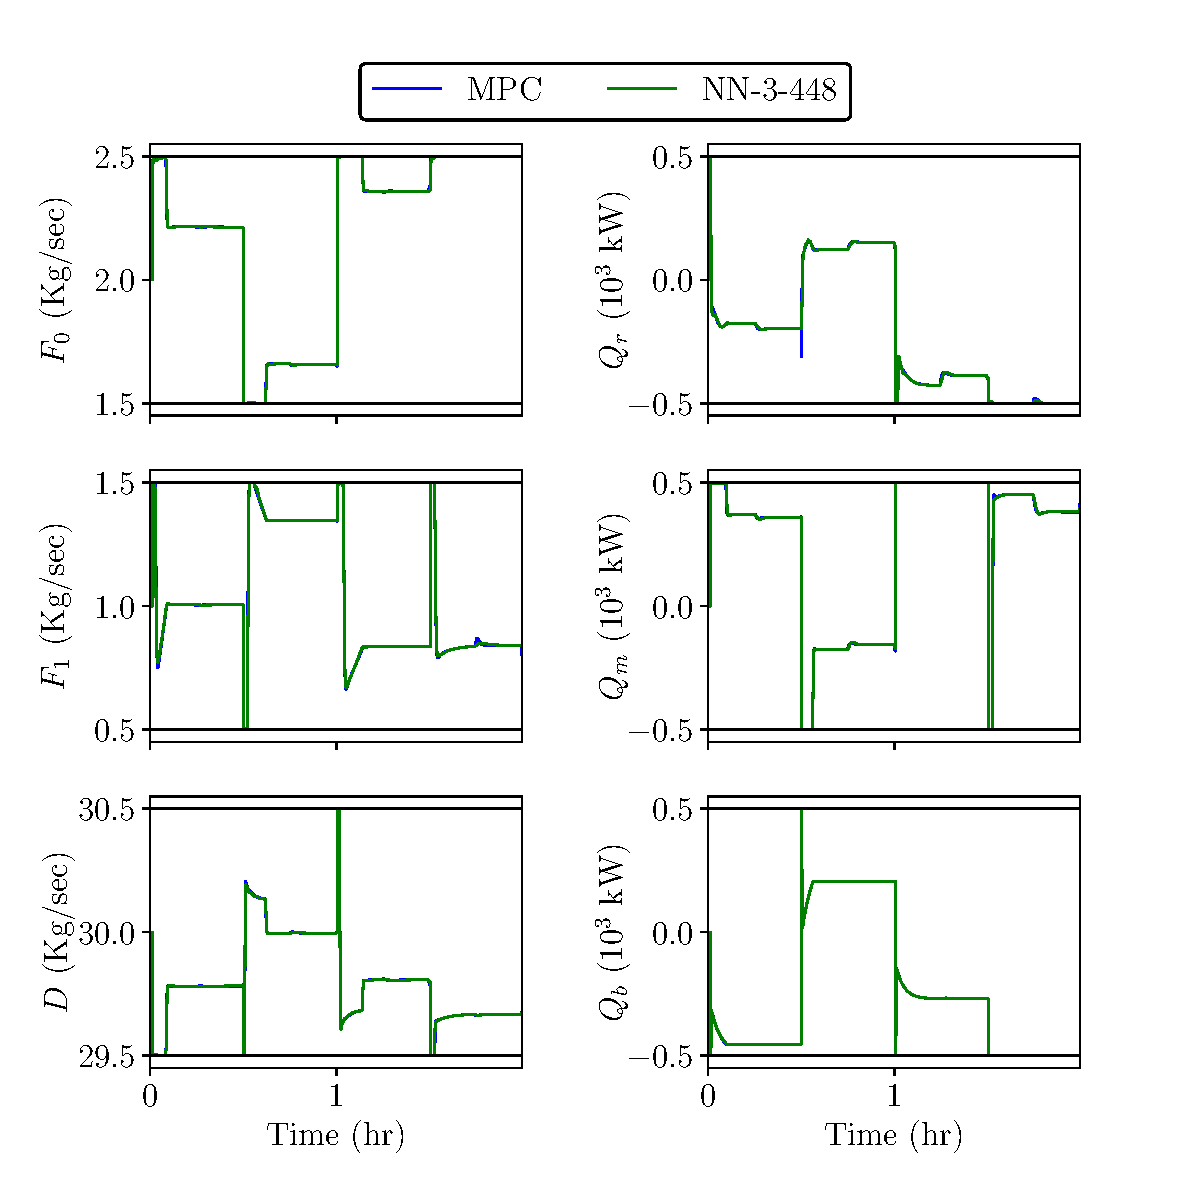
\includegraphics[page=1, 
		width=0.7\textwidth, 
        height=0.5\textheight]{cstrs_comparision_plots.pdf}    
        \caption{Transient closed-loop actuator trajectories of the CSTRs with 
        flash separator example with the NN and optimal MPC controllers.}   
    \label{fig:cl_cstrs_inputs}
\end{figure*}

\begin{figure*}[!h]
    \centering
	\includegraphics[page=2, 
		width=0.7\textwidth, 
		height=0.5\textheight]{cstrs_comparision_plots.pdf}
        \caption{Transient closed-loop controlled measurement 
        trajectories of the CSTRs with 
        flash separator example with the NN and optimal MPC controllers.}      \label{fig:cl_cstrs_outputs}
\end{figure*}

The robustness property of NN controllers 
is now presented. The optimal MPC controller
designed for a nominal linear system ignoring disturbances
is known to be inherently robust to bounded state 
estimation errors and disturbances
\citep*{heath:wills:2005, pannocchia:rawlings:wright:2011}. 
The approximation
error of the MPC feedback law by a NN can be viewed 
as an additional disturbance, and the existing
input-to-state stability
results \citep*{sontag:wang:1995} are used to establish the 
allowable approximation error in the NN for 
the NN controller to be robust to disturbances. 
Theorem \ref{thm:nnrobustness} states this 
allowable approximation error and the size 
of disturbances for which the NN controller is robust.

The problem of steering the state of the linear 
system (\ref{eq:ltimodel}) 
to one fixed steady state ($x_s, u_s$) is considered. 
For the analysis in this section, 
the state and control are transformed in deviation variables 
as $x := x - x_s$ and $u := u -u_s$,
and define the control problem as regulation to the origin.
The optimal MPC control law is denoted as $\kappa_N(x)$, 
and the NN control law as
$\kappa_{NN}(x) = \kappa_N(x) + e_{NN}(x)$, in which 
$e_{NN}(x)$ is the approximation error 
of the optimal control law by the network. Assume 
in the analysis that the target steady state 
is such that the unconstrained linear quadratic regulator (LQR)
satisfies the actuator constraints 
in a small neighborhood near the origin. 

As reviewed in \cite*{mayne:rawlings:rao:scokaert:2000},
the nominal stability of MPC can be established
using the optimal cost function ($V_N^0(x)$) of the QP
as a Lyapunov function.
The region of attraction of the closed-loop system 
$x^+ = Ax + B\kappa_N(x)$ when no hard terminal region 
constraint \citep*{limon:alamo:salas:camacho:2006}  
is included in the QP can be characterized
as $\mathcal{X}_N = \textnormal{lev}_{Nd + \tau} \ V_N^0(x)$.
In which, $\tau$ is a level
set parameter of the terminal region chosen as
$\bbX_f = \textnormal{lev}_{\tau} \ x'Px$, and $d > 0$
is a constant such that $\ell(x, u) \geq d$ for all 
$x \in \bbR^n \setminus \bbX_f$ and 
$\underline{u} \leq u+u_s \leq \overline{u}$.
The parameter $\tau$ is chosen small enough such that
the unconstrained LQR satisfies the actuator constraints 
for all $x \in \bbX_f$. The optimal cost 
function is continuous and satisfies 
$c_1\vert x \vert^2 \leq V_N^0(x) \leq c_2\vert x \vert^2$
and $V_N^0(x^+) - V_N^0(x) \leq -c_1\vert x \vert^2$ 
for some $c_2 \geq c_1 > 0$.

Assume that a state estimate ($\hat{x}$) is
used by the NN to compute the control. 
To analyze robustness, the following perturbed
linear system is considered
\begin{align} \label{eq:perturbed_sys}
    \hat{x}^+ = A\hat{x} + B\kappa_N(\hat{x}) + Be_{NN}(\hat{x}) + w - Ae + e^+
\end{align}
in which $\hat{x} = x + e$ is the state estimate, 
$w$ is a process disturbance, 
and $e$, $e^+$ are the state estimation errors at the 
current and next timestep respectively. 
We use $\phi_d(k;\hat{x})$ to denote a 
solution of the perturbed system 
at time $k$ starting from an initial state $\hat{x}$,
and $\phi(k;x)$ to denote a solution 
of the nominal system when the state estimation errors and process
disturbances are zero starting 
from an initial state $x$.

\begin{thm} \label{thm:nnrobustness}
For all $ 0 < \rho \leq Nd + \tau$, 
there exist constants $\delta_1, \delta_2, \delta_3 > 0$, 
functions $\beta(\cdot) \in \mathcal{K} \mathcal{L}$
and $\alpha_e(\cdot) , \alpha_w(\cdot), \alpha_{n}(\cdot) \in \mathcal{K}$,
such that for all disturbance sequences
satisfying $\vert\vert \mathbf{e}_{k+1} \vert\vert \leq \delta_1$,
$\vert\vert \mathbf{w}_k \vert\vert \leq \delta_2$,
and $\vert e_{NN}(\hat{x}) \vert \leq \delta_3$,
for all $\hat{x}$ in the set $S := \textnormal{lev}_{\rho} \ V_N^0(\hat{x})$,
we have the following bound 
$\vert \phi_d(k; \hat{x}) \vert \leq \beta(\vert \hat{x} \vert, k) 
+ \alpha_e(\vert \vert\mathbf{e}_{k+1} \vert \vert) + 
\alpha_w(\vert \vert \mathbf{w}_k \vert \vert) + 
\alpha_n(\bar{e}_{NN})$, 
in which 
$\bar{e}_{NN} = \textnormal{max}_{\hat{x} \in S} \vert e_{NN}(\hat{x}) \vert$.
\end{thm}

The proof of this theorem along with the required 
input-to-state stability definitions is provided 
in Appendix \ref{app:theorem1}.
In the nominal case, 
the disturbance sequences $\mathbf{e}$ and $\mathbf{w}$ are zero.
The closed-loop states in this case have the bound
$\vert \phi(k; x) \vert \leq \beta(\vert x \vert, k) + 
\alpha_n(\bar{e}_{NN})$. Any additional value of 
the NN training is to reduce the worst 
approximation error ($\bar{e}_{NN}$) 
in the state space of interest and 
strengthen the bounds on the closed-loop states. 

\section{Simulation studies} \label{sec:simulation_studies}

In this section, two case studies are presented 
which demonstrate the 
scalability of the proposed NN design approach.
The closed-loop performance of NNs and computational benefits over 
online QP based MPC are analyzed in these case studies.
After the offline design of NNs,
two types of validation simulations 
are performed: (i) with setpoints 
and disturbances not present in the training 
data but within the same range of values used to 
generate the training data, (ii) with extra setpoint 
signals assumed to be
unknown during the offline network design phase.
Both these types of simulations are conducted to 
analyze the interpolation and extrapolation 
abilities of the NNs, and are referred subsequently as 
simulations with expected and unexpected plant behaviors.

The closed-loop performance of the 
following alternative and 
equivalently fast controllers as NNs are also compared
in the validation simulations.
a) steady state controller (SS): the solution
of the target selector is directly applied to the plant 
$u = u_s$, b) saturated linear quadratic regulator (satK):
the unconstrained LQR gain 
$K$ is computed and used in the control law 
$u = \textnormal{sat}(K(x-x_s) + u_s, \underline{u}, \overline{u})$,
c) short horizon controller (SH): an MPC problem
with a short control horizon is solved online, 
d) Unstructured NN (NN-UNS): a standard feedforward network is 
trained with the triple ($x, x_s, u_s$) as the input
and then used as the feedback controller online.

\begin{figure}[h]
    \centering
    \includegraphics[width=0.5\textwidth, 
                     height=0.22\textheight]{cstrs_with_flash.pdf}
    \caption{Schematic of the CSTRs with a flash separator model}
    \label{fig:schematic_cstrs}
\end{figure}

To gauge the performance of NNs in 
the validation simulations, the offline
computational effort required to build the NNs, 
and the memory required for the deployment of NNs,
the following metrics are examined:

\begin{itemize}
    \item Controller performance index
    \begin{align*}        
    \Lambda_k = \dfrac{1}{k}\sum_{t=1}^{k} & \big(\vert x(t) - x_{s} (t) \vert^2_{Q} \\
        & + \vert u(t) - u_{s} (t) \vert^2_{R} + \vert \Delta u(t) \vert^2_{S}\big)         
    \end{align*}
    \item \% Performance loss = $100(\Lambda^{\textnormal{F}}_{N_{t}} - \Lambda^{\textnormal{MPC}}_{N_{t}})/\Lambda^{\textnormal{MPC}}_{N_{t}}$
    \item Average and worst-case speedups
    \item Data generation and NN training times
    \item Memory required to store the weights of the NNs
\end{itemize}
Here, $N_t$ is the number of simulation time steps,  
$\Lambda^{\textnormal{F}}_{N_{t}}$ and 
$\Lambda^{\textnormal{MPC}}_{N_{t}}$
are the average stage costs obtained 
at the end of the simulation period by the 
fast controllers and the MPC controller.
The data generation and online timing comparisons are 
performed on a computing cluster that has 
several multi-core CPUs of clock speed 2.4GHz. 
The NN trainings are performed on a 
Tesla V100-SXM2 GPU that has 32 GB memory.

\begin{table*}[t]
    \caption{Summary of the simulation study for the
    CSTRs with a flash separator example.}   
    \begin{tabular}{ |c|c|c|c|c|c|c|c| }
        \hline
        Controller & \thead{Structured network \\ architecture} & 
        \thead{Number of \\ Parameters} & 
    \thead{Memory \\ footprint \\ (mB)} & \thead{Training \\ time \\ (min)} &
        \thead{\% Performance\\ losses \\ Expected, Unexpected \\ plant behaviors} & \thead{Average \\ speedup} & \thead{Worst case \\ speedup} \\
        \hline
    SS &  &  & &  & 85.18\%, 106.39 \% &  & \\ 
    satK &  &  &  &  & 41.03\%, 27.61 \% & $2.47 \times 10^5$ & 
    $3.07 \times 10^5$ \\ 
    SH &  &  &  &  & 1.61\%, 2.46 \% & $3.75 \times 10^3$ & $8.4 \times 10^1$ \\ 
    NN-UNS &  &  &  &  & 80.49\%, 73.29 \% & $9.31 \times 10^4$ & $4.99 \times 10^3$ \\ 
NN-3-448 & [72, 448, 448, 448, 6] & $1.10 \times 10^5$ & 0.84 & 13.02 & 0.28 \%, 5.57 \% & $5.26 \times 10^4$ & $1.45 \times 10^3$ \\ 
NN-3-480 & [72, 480, 480, 480, 6]  & $1.26 \times 10^5$ & 0.96  & 12.51 & 0.34 \%, 7.58\% & $5.09 \times 10^4$ & $1.53 \times 10^4$ \\ 
NN-3-512 & [72, 512, 512, 512, 6]  & $1.42 \times 10^5$ & 1.08  & 12.77 & 0.16 \%, 5.90 \% & $4.62 \times 10^4$ & $1.58 \times 10^4$ \\ 
        \hline
       \end{tabular}
       \label{table:cstrs}      
\end{table*}

\begin{figure*}[!h]
    \includegraphics[page=31,
        width=0.5\textwidth, 
        height=0.28\textheight]{cstrs_comparision_plots.pdf} \hfill
    \includegraphics[page=34,
        width=0.5\textwidth, 
        height=0.28\textheight]{cstrs_comparision_plots.pdf} \vfill
    \vspace{-0.1in}
    \begin{center}\includegraphics[page=33,
        width=0.5\textwidth, 
        height=0.28\textheight]{cstrs_comparision_plots.pdf}
    \end{center}
    \vspace{-0.2in}
    \caption{Simulation statistics for the  
    CSTRs with a flash separator example. Data requirement to obtain accurate NN controllers (top left), online computation times of the NNs and 
    MPC controller (top right), 
    and the controller performance index obtained with the NNs, 
    SS, satK and MPC controllers (center bottom).}	
    \label{fig:cstrs_statistics}
\end{figure*}

\subsection{CSTRs with a flash separator}
For the first example, the two 
stirred tank reactors in series with a flash separator
depicted in Figure \ref{fig:schematic_cstrs} 
is considered as the plant.
In both the CSTRs, a desired product $B$ is produced 
with the reaction $A \rightarrow B$, and an undesired 
product $C$ is produced with the reaction $B \rightarrow C$. 
The reactant $A$ is the major component in the 
feed streams supplied to the 
reactors. After the second CSTR, the reaction mixture is 
sent to the non-adiabatic flash that separates the reactant $A$
from the product $B$. The $A$ rich vapor phase 
is recycled back to the first CSTR. 
The plant is simulated using the set of 
nonlinear ordinary differential equations (ODEs) available in 
\cite*{venkat:2006}, Appendix.
The model has 12 states 
($H_r, x_{Ar}, x_{Br}, T_r, 
H_m, x_{Am}, x_{Bm}, T_m, H_b, x_{Ab}, x_{Bb}, T_b$),
6 control inputs 
($F_0, F_1, D, Q_r, Q_m, Q_b$), and 5 disturbances
($x_{A0}, x_{A1}, x_{B0}, x_{B1}, T_0$).
The controlled measurements with setpoints are the heights
and temperatures of the three units, and we
assume that all the states are measured for this example. 
The sample time for the measurements is chosen as 10 seconds. 
The parameter values used to simulate the ODEs for the plant, 
the actuator constraints, and the bounds of the controlled 
measurements and disturbances used for the data generation 
and validation simulations are 
shown in Table \ref{table:cstrs_pars}, Appendix \ref{app:cstrs_pars}.

A linear discrete time model with the chosen sample time
is obtained at the steady state shown in the Table 
\ref{table:cstrs_pars}.
This model, inputs and outputs are scaled 
for the MPC controller such that the input 
constraints satisfy
$\overline{u} - \underline{u} = \mathbf{2}$.
The tuning parameters and 
control horizon length for the regulator are chosen as
$Q = 10^3 C'C$, $R = 0.1 I$, $S = 0.1 I$, 
and $N = 450$.
A total $1.5 \times 10^5$ samples of 
($x, u_{-1}, x_s, u_s, \kappa_N(\cdot)$) 
is generated for NN training, parallelized in 100 
separate offline simulations. The time consumed 
for this data generation step was 4.2 hours.
The setpoint of the 
height of the second CSTR ($H_m$) is assumed 
to be fixed during this data generation process, 
and is included as an additional setpoint
in the validation simulations for the 
unexpected plant behavior case.

Three structured NN architectures 
are considered. Each NN
has three hidden layers with 
448 (NN-3-448), 480 (NN-3-480), 
and 512 (NN-3-512)
nodes in each hidden 
layer respectively. For validation simulations, 
two sets of setpoint and disturbance signals 
with 24 setpoint changes and 48 disturbance changes 
are generated for 4320 timesteps (12 hours), 
each for the expected and unexpected 
plant behavior cases. 
The short horizon MPC controller is constructed with a 
horizon length of $N = 10$, and the architecture 
of the unstructured NN considered 
is three hidden layers with 224 nodes in each hidden layer. 
An additional scaling of $x$ and $x_s$ is performed for the 
NN training as $x := 2x/(x_{\textnormal{max}} - x_{\textnormal{min}})$ and 
$x_s := 2x_s/(x_{\textnormal{max}} - x_{\textnormal{min}})$,
in which $x_{\textnormal{max}}$ and $x_{\textnormal{min}}$
are the maximum and minimum values of the state 
observed in the training data.
This scaling is also performed in real time 
when the NN is used to compute the actuator move.

First, the amount of data required to obtain an accurate 
NN controller is studied. To this aim, NNs with 
the three chosen architectures are trained with 
incremental increases of 
$10^4$ training samples starting from $4 \times 10^4$
to $1.5 \times 10^5$ samples. 
A batch size of 1024 samples is used in Adam, 
and all the NNs are trained for 2000 epochs. 
The NNs after training are used in validation simulations
with the setpoint and disturbance
signals generated for the expected plant behavior
case. The closed-loop performance is 
compared with the optimal MPC 
controller and the $\%$ performance loss obtained
is plotted in Figure \ref{fig:cstrs_statistics} (top left)
as a function of the number of training samples.
All the trained NNs provide less than $1 \%$ loss in 
this performance metric after training with 
about $9 \times 10^4$ samples. The best $\%$ performance
loss obtained by the NNs is summarized in
Table \ref{table:cstrs}. 

Second, the above trained NNs with the best 
performance losses are used in validation simulations
with the setpoint and disturbance signals generated 
for the unexpected plant behavior case. The 
$\%$ performance losses obtained in these simulations 
are also summarized in the Table \ref{table:cstrs},
and the performance degrades from 
less than $1\%$ to $5-8\%$. 
This deterioration in the performance is due to some unseen
($x, u_{-1}, x_s, u_s$) encountered in real-time by the NN
resulting from the setpoint changes of the height 
of the second CSTR, which was assumed to be fixed 
during the data generation. 
These simulations illustrate that one must not 
expect the NNs to extrapolate outside the training data.
The practical implication of this study is that 
all possible plant scenarios with the 
setpoints and disturbances 
must be identified a-priori the deployment of NNs, and 
should be used to generate the training data.

\begin{table*}[t]
    \caption{Summary of the simulation study for the 
    industrial crude distillation unit example.}
    %\centering
\begin{tabular}{ |c|c|c|c|c|c|c|c| }
          \hline
          Controller & \thead{Structured network \\ architecture} & 
          \thead{Number of \\ Parameters} & 
          \thead{Memory \\ footprint \\ (mB)} & \thead{Training \\ time \\ (min)} &
          \thead{\% Performance\\ loss} & \thead{Average \\ speedup} & \thead{Worst case \\ speedup} \\
          \hline
      SS &  &  & &  & 120.59 \% &  & \\ 
  satK &  &  &   &  & 13.07 \% & $4.83 \times 10^5$ & $1.51 \times 10^5$ \\ 
  SH &  &  &  &  & 1.56 \% & $6.66 \times 10^3$  & $2.51 \times 10^3$ \\ 
  NN-3-1664 & [1072, 1664, 1664, 1664, 32] & $1.85 \times 10^6$ & 14.18 & 52.66 & 0.29 \% & $1.52 \times 10^4$ & $6.57 \times 10^3$  \\ 
  NN-3-1792 & [1072, 1792, 1792, 1792, 32]  & $2.11 \times 10^6$ & 16.15  & 55.27 & 0.43 \% & $1.33 \times 10^4$ & $5.25 \times 10^3$ \\ 
  NN-3-1920 & [1072, 1920, 1920, 1920, 32]  & $2.39 \times 10^6$ & 18.24  & 59.24 & 0.59 \% & $1.18 \times 10^4$ & $4.48 \times 10^3$ \\ 
  NN-3-2048 & [1072, 2048, 2048, 2048, 32]  & $2.68 \times 10^6$ & 20.46  & 66.58 & 0.48 \% & $1.09 \times 10^4$ & $3.54 \times 10^3$\\ 
\hline
\end{tabular}
\label{table:cdu}      
\end{table*}

\begin{figure*}[!h]
    \includegraphics[page=41,
        width=0.5\textwidth, 
        height=0.28\textheight]{cdu_comparision_plots.pdf} \hfill
    \includegraphics[page=43,
        width=0.5\textwidth, 
        height=0.28\textheight]{cdu_comparision_plots.pdf} \vfill
    \vspace{-0.1in}
    \begin{center}\includegraphics[page=42,
        width=0.5\textwidth, 
        height=0.28\textheight]{cdu_comparision_plots.pdf}\end{center}
    \vspace{-0.2in}
    \caption{Simulation statistics for the industrial 
    crude distillation unit example. Data requirement to obtain accurate NN controllers (top left), online computation times of the NNs and 
    MPC controller (top right), 
    and the controller performance index obtained with the NNs, 
    satK and MPC controllers (center bottom).}	
    \label{fig:cdu_statistics}
\end{figure*}

\begin{figure}[!h]
    \centering
    \includegraphics[width=0.45\textwidth, 
                     height=0.25\textheight]{cdu.pdf}
    \caption{Schematic of the industrial crude distillation unit model}
    \label{fig:schematic_cdu}
\end{figure}

Third, the transient closed-loop 
performance of the trained NNs is examined
for one particular validation 
simulation for the expected plant behavior case. 
Figures \ref{fig:cl_cstrs_inputs} and \ref{fig:cl_cstrs_outputs}
show the transient actuator 
and controlled measurements obtained with the NN-3-448 and 
optimal MPC controllers for a simulation period of 2 hours.
The Figure \ref{fig:cstrs_statistics} (center bottom)
shows the transient values of the controller performance index
obtained in this validation simulation
with the three structured NNs, SS, satK 
and optimal MPC controllers for the full 
simulation period of 12 hours. The closed-loop 
performance obtained using NNs is almost same as the optimal MPC 
controller and the degradation in the performance 
is quantified with the $\%$ performance loss metric.

Fourth, the online computational benefits of NNs 
over the QP based MPC is analyzed. The Figure 
\ref{fig:cstrs_statistics} (top right)
shows a histogram of online computation times
of the NNs and QP solver in one validation
simulation. The average and worst-case speedups
obtained using NNs are summarized in the 
Table \ref{table:cstrs}. The QP solver takes 
about 8 to 13 seconds in this example and all the 
NNs compute the control in just 0.1 to 4
milliseconds, and are easily deployable in the 
sample time of 10 seconds.

The $\%$ performance loss 
obtained using the four heuristic controllers, 
their corresponding speedups, maximum time required to 
train each NN, number of parameters in each NN, 
and the memory required to store  
the weights of the NNs is summarized in the 
Table \ref{table:cstrs}. The 
$85 \%$ performance loss 
reported for the unstructured
NN corresponds to training with $1.5 \times 10^5$  
samples and the performance is unacceptable 
for an industrial application. 
The noticeable performance improvement with the
structured NNs is because the control law 
is exactly the same as the optimal feedback law
at steady-states, and that simplifies
the optimal feedback law approximation problem
since the training process only has to improve the 
NN control law for the transient conditions. 

\subsection{Large-scale crude distillation unit}

The scalability of the proposed NN design 
approach is next demonstrated on an industrial crude 
distillation unit model \citep*{pannocchia:rawlings:wright:2007} 
with 252 states, 32 controls, and 90 measurements. The 
schematic of this model is shown in Figure \ref{fig:schematic_cdu}, 
which is a typical crude unit found in petrochemical refineries.
The plant model is linear, input and outputs are scaled 
for the MPC regulator as in the previous example.
Only four measurements that represent 
the quality of the crude side products have setpoints, 
and five disturbances are used on the crude composition, 
fuel gas quality, and steam header pressure. 
The sample time for the measurements is 1 min. The tuning 
parameters and control horizon length for the 
MPC regulator are chosen as $Q = 2C'C$, $R = 0.1I$, 
and $N = 140$. A total $3.6 \times 10^5$ 
samples of ($x, x_s, u_s, \kappa_N(\cdot)$)
are generated for the NN training, parallelized over 
149 offline simulations. The time consumed 
for this data generation step was 
27.8 hours.

Four structured NN architectures 
are considered for this example. Each NN
has three hidden layers, with 
1664 (NN-3-1664), 1792 (NN-3-1792), 
1920 (NN-3-1920), and 2048 (NN-3-2048) 
nodes in each hidden layer respectively. 
For the validation simulations, one set of
setpoint and disturbance signals for the expected 
plant behavior case is generated
with 24 setpoint changes and 48 disturbance changes 
for 2880 timesteps (2 days). 
The short horizon MPC controller is constructed with a 
horizon length of $N = 3$. 
The states and target steady-states 
($x$, $x_s$) are scaled for the NN training
as in the previous example. 

Figure \ref{fig:cdu_statistics} shows the 
statistics for the simulation study performed for this 
example.
The data requirement to obtain 
an accurate NN controller is shown in top left.
The batch size 
in Adam was chosen as 2048 samples, and all the NNs 
are trained for 1500 epochs.
The transient controller performance index 
for one validation simulation
obtained with the four structured NNs,
satK, and MPC controllers is shown in center bottom.
The top right plot shows the 
histogram of online computation times 
of the NNs and QP solver.
Table \ref{table:cdu} gives a summary of 
the maximum time required to train the NNs, number of parameters
in each NN, memory footprint of the NNs, and 
the $\%$ performance loss metric obtained by 
the structured NNs, SS, satK, and SH 
controllers in the validation simulations. 

The offline data generation and training times 
for the NNs shows that this large-scale example
is tractable with the proposed NN approach.
This large example is challenging, 
since on average the QP solver CVXOPT requires 
35 seconds, and 
47 seconds in the worst-case. By comparison,  
all the NNs execute MPC in about 2 
to 7 milliseconds.
As observed from the plot of the transient controller 
performance index, the performance 
degradation by the NNs relative to 
the optimal MPC controller is negligible.
The sampling of the state space with 
the setpoint and disturbance signals
for one particular operational scenario,
combined with the offset-free NN structure
are the key steps for scalability in this example. 

\section{Conclusion} \label{sec:conclusion}
Neural networks have been demonstrated 
to approximate the MPC feedback law
for treating large-scale, linear MPC applications
that may be out of reach with QP solvers. 
The proposed no online optimization based
methods to date in the literature such as storing 
the entire MPC feedback law 
and sampling the large dimensional state space 
for the NN training are not tractable for the problems 
considered in this article.

The key features for the scalability of the proposed approach 
are the structure of NN and data generation for only
typical plant operational scenarios. 
The NN design approach was demonstrated to scale on an
industrial crude distillation unit model with state and
control dimensions of 252 and 32 respectively, and 
a control-sample horizon length of 140. 
After the offline design phase, NNs execute MPC 
about three to five orders of magnitude faster than an 
available QP solver 
with less than 1$\%$ performance degradation in the closed-loop.
The deployment decision of the NNs 
must be based on the ability to reliably identify 
and sample the anticipated plant operational scenarios 
with setpoints and large magnitude disturbances
that may change for a reasonable duration of operation.
Parallel computing can be used for
the offline data generation step if
solving QPs for each sampled state starts to take 
excessive amounts of time.
After the training process, 
the NNs are easily deployable on memory constrained 
hardware. We established conditions under which the 
NN controllers are robust to state estimation errors 
and process disturbances,
provides some theoretical support 
to practitioners interested in the deployment of NNs. 

\section*{Acknowledgement}
%The authors acknowledge Professor Stephen J. Wright 
%at the University of Wisconsin, Madison
%for helpful discussions on machine learning topics and providing 
%a detailed feedback on this article.
The funding for this work was provided by the industrial
members of the Texas-Wisconsin-California Control 
Consortium (TWCCC).
The computational facilities purchased with funds from the National Science Foundation (CNS-1725797) and 
administered by the Center for Scientific Computing (CSC) was used for the simulation 
studies presented in this article. 
The CSC is supported by the California NanoSystems Institute and the Materials 
Research Science and Engineering Center 
(MRSEC; NSF DMR 1720256) at UC Santa Barbara.

%% New version of the num-names style
\bibliographystyle{elsarticle-num-names}
\bibliography{abbreviations,articles,books,unpub,proceedings}

\section*{Appendix}
\renewcommand{\thesubsection}{\Alph{subsection}}

\subsection{Proof of Theorem \ref{thm:nnrobustness}} \label{app:theorem1}

We use the following
definitions of
robust positive invariance of a set
with respect to disturbances, 
input-to-state stability (ISS), ISS-Lyapunov function,
and the available result 
on the ISS property of a system if it admits 
an ISS-Lyapunov function
(\cite*{jiang:wang:2001, 
rawlings:mayne:diehl:2017}, Appendix B).

\begin{definition} \label{def:robust_pos_invariance}
(Robust positive invariance). A closed set $X$ is 
robustly positive invariant for the system $x^+ = f(x, w)$, 
$w \in \bbW$ if $x \in X$ 
implies $f(x, w) \in X$ for all $w \in \bbW$.
\end{definition}

\begin{definition} \label{def:iss}
(Input-to-state stability (ISS)). $\bbW$ is a compact 
set containing the origin and that $X$ is a closed robustly
positive invariant set for the 
system $x^+ = f(x, w)$, $w \in \bbW$. This
system is ISS in $X$ if there exist functions 
$\beta(\cdot) \in \mathcal{K}\mathcal{L}$ and 
$\sigma(\cdot) \in \mathcal{K}$, such that for all
$x \in X$ and $w(i) \in \bbW$, $i \in \bbI_{0:k-1}$, 
$\vert \psi(k; x, \mathbf{w}_k) \vert \leq \beta(\vert x\vert, k) 
+ \sigma(\vert \vert \mathbf{w}_k\vert \vert)$, in which 
$\psi(k; x, \mathbf{w}_k)$ is the solution of the system 
at time $k$, starting from an initial state $x$, and with the
disturbance sequence $\mathbf{w}_k$ affecting the system.
\end{definition}

\begin{definition} \label{def:iss_lyapunov_func}
(ISS-Lyapunov function). A function $V : X \rightarrow \bbR_{\geq 0}$
is an ISS-Lyapunov function in $X$ for the system $x^+ = f(x, w)$, $w \in \bbW$
if there exist functions $\alpha_1(\cdot), \alpha_2(\cdot), \alpha_3(\cdot) 
\in \mathcal{K}_{\infty}$ and $\sigma(\cdot) \in \mathcal{K}$
such that for all $x \in X$ and $w \in \bbW$
\begin{align*}
    \alpha_1(\vert x \vert) \leq & V(x) \leq \alpha_2(\vert x \vert) \\
    V(f(x, w)) &- V(x) \leq -\alpha_3(\vert x \vert) + \sigma(\vert w \vert)
\end{align*}
\end{definition}

\begin{prop} \label{prop:lyapunov_implies_iss}
(ISS-Lyapunov function implies ISS). $\bbW$ is a compact
set containing the origin and that $X$ is a closed robustly
positive invariant set for $x^+ = f(x, w)$, $w \in \bbW$. If 
$f(\cdot)$ is continuous and there exists a continuous 
ISS-Lyapunov function in $X$ for the system $x^+ = f(x, w)$, $w \in \bbW$, 
then the system is ISS in $X$.
\end{prop}

Additionally, we require the following two 
useful propositions from 
\cite*{allan:bates:risbeck:rawlings:2017} and 
\cite*{rawlings:ji:2012},
to bound values of continuous functions and an
inequality for $\mathcal{K}$ functions respectively.

\begin{prop} \label{prop:continuous_funcs}
    Let $C \subseteq D \subseteq \bbR^n$, $C$ compact, 
    $D$ closed, and $f : D \rightarrow \bbR^n$ continuous.  
    Then there exists a $\sigma(\cdot) \in \mathcal{K}_{\infty}$,
    such that for all $x \in C$ and $y \in D$, we have that 
    $\vert f(x) - f(y) \vert \leq \sigma(\vert x-y \vert)$.
\end{prop}
    
\begin{prop} \label{prop:Kfunction_inequality}
    Let $\sigma(\cdot) \in \mathcal{K}$, the following holds 
    for all $a_i \in \bbR_{\geq 0}$, $i \in \bbI_{1:n}$ 
    \begin{align*}
        \sigma(a_1 + a_2 + \cdot \cdot + a_n) \leq \sigma(na_1) + 
        \sigma(na_2) + \cdot \cdot + \sigma(na_n)
    \end{align*}    
\end{prop}

\textbf{Proof of Theorem \ref{thm:nnrobustness}:}
We proceed in two steps. First, 
we show that there exist constants $\delta_1, \delta_2, \delta_3 > 0$
such that the set $S$ is robustly positive invariant. Then, we 
show that $V_N^0(\hat{x})$ is an ISS Lyapunov function for 
the perturbed system \eqref{eq:perturbed_sys} on this set $S$. Denote 
$\tilde{x}^+ = A\hat{x} + B\kappa_N(\hat{x})$ as the nominal 
state evolution using the optimal MPC controller, 
and $d(k) = [ e_{NN}(\hat{x}(k))'B', w(k)', e(k)', e(k+1)']'$
as the combination of all the disturbances at a given time $k$. 

To show robust positive invariance of $S$,  
we establish that if $V_N^0(\hat{x}) \leq \rho$, 
then $V_N^0(\hat{x}^+) \leq \rho$.
Since the optimal 
cost function ($V_N^0(\hat{x})$) is continuous,
using $\bbR^n$ as the closed set ($\hat{x}^+ \in \bbR^n$) 
and $S$ as the compact set ($\tilde{x} \in S$),
from proposition \ref{prop:continuous_funcs} we have
for some $\sigma_1(\cdot) \in \mathcal{K}_{\infty}$
\begin{align}
    \vert V_N^0(\hat{x}^+) - V_N^0(\tilde{x}^+) \vert &\leq 
    \sigma_1(\vert \hat{x}^+ - \tilde{x}^+ \vert)  \nonumber  \\
    &\leq 
   \sigma_1(\vert B e_{NN}(\hat{x}) \vert + \vert w \vert 
   \nonumber \\
   & + \vert A\vert\vert e \vert +  \vert e^+ \vert) \nonumber \\
     &\leq 
   \sigma_1(\vert d \vert + \vert d \vert + \vert A \vert\vert d \vert + \vert d \vert) := \sigma_2(\vert d \vert)
   \label{eq:optimal_cost_bound}
\end{align}
in which $\sigma_2(s) := \sigma_1(\vert A\vert s +3s)$, and the last inequality 
follows because $\vert a \vert \leq \vert [a', b']' \vert$, in which $a$ and $b$
are both vectors, and $\sigma_2(\cdot) \in \mathcal{K}_{\infty}$.
We partition $S$ in outer and inner parts based on 
the value of the optimal cost $V_N^0(\hat{x})$, and bound the 
combination of disturbances $d$ in each part 
such that $V_N^0(\hat{x}^+) \leq \rho$. \\
Case 1: $\rho/2 \leq V_N^0(\hat{x}) \leq \rho $. Using the 
upper bound on the optimal cost, we have 
$\rho/(2c_2) \leq \vert \hat{x} \vert^2$ for all $\hat{x}$ 
in this part of $S$. To analyze the worst-case disturbance, 
we have from the equation \eqref{eq:optimal_cost_bound} that 
$V_N^0(\hat{x}^+) \leq V_N^0(\tilde{x}^+) + \sigma_2(\vert d \vert) $.
From nominal MPC cost decrease, we obtain  
$V_N^0(\hat{x}^+) \leq V_N^0(\hat{x}) - c_1\vert \hat{x} \vert^2 + \sigma_2(\vert d \vert)$. Thus, if $\sigma_2(\vert d \vert) \leq \rho c_1/(2c_2)$, 
at all times in this outer part of $S$, we have 
$V_N^0(\hat{x}^+) \leq \rho$. \\
Case 2: $V_N^0(\hat{x}) \leq \rho/2 $. From 
equation \eqref{eq:optimal_cost_bound} and nominal MPC 
cost decrease, we have for this part of $S$ that 
$V_N^0(\hat{x}^+) \leq \rho/2 + \sigma_2(\vert d \vert)$.
Thus, if $\sigma_2(\vert d \vert) \leq \rho/2$, 
at all times in this inner part of $S$, we have 
$V_N^0(\hat{x}^+) \leq \rho$.

Therefore, if 
$\vert d \vert \leq \textnormal{min} \{ \sigma_2^{-1}(\rho c_1/(2c_2)), 
\sigma_2^{-1}(\rho/2)\} := \delta_{\textnormal{max}}$ 
at all times, then the set $S$ is 
robustly positive invariant. Since $c_1 \leq c_2$, 
$\delta_{\textnormal{max}} = \sigma_2^{-1}(\rho c_1/(2c_2))$.
The constants $\delta_1$ and $\delta_2$ are
$\delta_{\textnormal{max}}/4$ each, 
and $\delta_3$ is $\delta_{\textnormal{max}}/(4\vert B \vert)$.
The optimal MPC cost function satisfies
\begin{align*}
    V_N^0(\hat{x}^+) - V_N^0(\hat{x}) &\leq 
    -c_1\vert \hat{x} \vert^2 + \sigma_2(\vert d \vert)
\end{align*}
in the robustly positive invariant set $S$ and
the disturbance set $\vert d \vert \leq \delta_{\textnormal{max}}$.
Since the optimal cost function also satisfies the upper and lower bounds
$c_1\vert x \vert^2 \leq V_N^0(x) \leq c_2\vert x \vert^2$,
from the Definition \ref{def:iss_lyapunov_func},
it satisfies the requirements of an ISS-Lyapunov function.
Hence, using the Proposition \ref{prop:lyapunov_implies_iss}, 
the perturbed linear system \eqref{eq:perturbed_sys} is
ISS (Definition \ref{def:iss}), 
and there exist functions 
$\beta(\cdot) \in \mathcal{K}\mathcal{L}$ and 
$\sigma(\cdot) \in \mathcal{K}$, such that 
$\vert \phi_d(k; \hat{x}) \vert \leq \beta(\vert \hat{x} \vert, k) 
+ \sigma(\vert\vert \mathbf{d}_k\vert\vert)$. Using the Proposition
\ref{prop:Kfunction_inequality} and the definition of 
$d(k)$, we have 
\begin{align*}
    \vert \phi_d(k; \hat{x}) \vert & \leq \beta(\vert \hat{x} \vert, k)
    + \sigma(\vert B\vert\bar{e}_{NN} + \vert \vert \mathbf{w}_k \vert \vert
    + 2\vert \vert \mathbf{e}_{k+1} \vert \vert) \\
     & \leq \beta(\vert \hat{x} \vert, k) \\
    & +\sigma(3\vert B\vert\bar{e}_{NN}) + 
    \sigma(3\vert \vert \mathbf{w}_k \vert \vert)
    + \sigma(6\vert \vert \mathbf{e}_{k+1} \vert\vert)
\end{align*}
Therefore, the bound in the Theorem \ref{thm:nnrobustness} is established with 
$\alpha_e(s) := \sigma(6s)$, 
$\alpha_w(s) := \sigma(3s)$,
$\alpha_n(s) := \sigma(3\vert B\vert s)$, and 
$\alpha_e(\cdot), \alpha_w(\cdot), \alpha_n(\cdot) \in \mathcal{K}$.

\subsection{Parameters used in the CSTRs example} \label{app:cstrs_pars}

\renewcommand{\arraystretch}{1.1}
\begin{table}[!h]
    \centering
    \resizebox{\columnwidth}{!}{
    \begin{tabular}{|c|c|c|c|c|c|}
        \hline
        \multicolumn{6}{ |c| }{Parameters used to simulate the ODEs} \\
        \hline
        Parameter & Value & Unit & Parameter & Value & Unit\\
        \hline
        $\alpha_A$ & 3.5 &  & $k_m$ & 2.5 & \unit{m$^2$}\\ 
        $\alpha_B$ & 1.1 &  & $k_b$ & 1.5 & \unit{m$^2$} \\ 
        $\alpha_C$ & 0.5 &  & $\Delta H_1$ & -40 & \unitfrac{kJ}{kg} \\ 
        $\rho$ & 50 & \unitfrac{kg}{m$^3$} & $\Delta H_2$ & -50 
        & \unitfrac{kJ}{kg} \\ 
        $C_p$ & 3 & \unitfrac{kJ}{kg-K} & $E/R$ & 150 & \unit{K} \\ 
        $A_r$ & 0.3 & \unit{m$^2$} & $k^{\star}_1$ & $4 \times 10^{-4}$ & 
        \unit{sec$^{-1}$} \\ 
        $A_m$ & 2 & \unit{m$^2$} & $k^{\star}_2$ & $1.8 \times 10^{-6}$ & \unit{sec$^{-1}$} \\ 
        $A_b$ & 4 & \unit{m$^2$} & $T_d$ & 313 & \unit{K} \\ 
        $k_r$ & 2.5 & \unit{m$^2$} &  &  &  \\ 
        \hline       
        \multicolumn{6}{ |c| }{Actuator constraints ($\underline{u}, 
        \overline{u}$)} \\
        \hline
        $F_0$ & (1.5, 2.5) & \unitfrac{kg}{sec} & 
        $Q_r$ & (-500, 500) & \unit{kW} \\ 
        $F_1$ & (0.5, 1.5) & \unitfrac{kg}{sec} & 
        $Q_m$ & (-500, 500) & \unit{kW} \\ 
        $D$ & (29.5, 30.5) & \unitfrac{kg}{sec} & 
        $Q_b$ & (-500, 500) & \unit{kW} \\ 
        \hline
        \multicolumn{6}{ |c| }{Setpoint bounds ($\underline{r}_{sp}, 
        \overline{r}_{sp}$)} \\
        \hline
        $H_r$ & (158.8, 168.8) & \unit{m} & 
        $T_r$ & (303, 323) & \unit{K} \\ 
        $H_m$ & (169.2, 179.2) & \unit{m} & 
        $T_m$ & (310, 316) & \unit{K} \\ 
        $H_b$ & (2.2, 4.2) & \unit{m} & 
        $T_b$ & (303, 323) & \unit{K} \\ 
        \hline
        \multicolumn{6}{ |c| }{Disturbance bounds ($\underline{d}, 
        \overline{d}$)} \\
        \hline
        $x_{A0}$ & (0.7, 0.85) & & 
        $x_{B1}$ & (0, 0.15) & \\ 
        $x_{B0}$ & (0, 0.15) & & 
        $T_0$ & (305, 321) & \unit{K} \\ 
        $x_{A1}$ & (0.7, 0.85) & & 
         & & \\ 
        \hline       
        \multicolumn{6}{ |c| }{Steady state used for linearization 
        ($x_s, u_s, d_s$)} \\
        \hline
        $H_r$ & 163.8 & \unit{m} & $F_0$ & 2 & \unitfrac{kg}{sec} \\ 
        $x_{Ar}$ & 0.40 &  & $F_1$ & 1 & \unitfrac{kg}{sec} \\ 
        $x_{Br}$ & 0.54 &  & $D$ & 30 & \unitfrac{kg}{sec} \\ 
        $T_r$ & 313.1 & \unit{K} & $Q_r$ & 0
        & \unit{kW} \\ 
        $H_m$ & 174.2 & \unit{m} & $Q_m$ & 0 & \unit{KW} \\ 
        $x_{Am}$ & 0.37 &  & $Q_b$ & 0 & 
        \unit{kW} \\ 
        $x_{Bm}$ & 0.58 & & $x_{A0}$ & 0.8 &  \\ 
        $T_m$ & 313.7 & \unit{K} & $x_{B0}$ & 0.1 & \\ 
        $H_b$ & 3.24 & \unit{m} &  $x_{A1}$&  0.8&  \\ 
        $x_{Ab}$ & 0.15 &  & 
        $x_{B1}$ & 0.1 &  \\ 
        $x_{Bb}$ & 0.73 &  & 
        $T_0$ & 313 & \unit{K} \\ 
        $T_b$ & 313.7 & \unit{K} & 
         & & \\ 
        \hline
    \end{tabular}}
    \caption{Parameters used in the ODEs to 
simulate the plant in the CSTRs in series
with a flash separator example, 
actuator constraints, 
setpoint and disturbance bounds, 
and the steady state used to obtain the 
linear model for the MPC controller.}
\label{table:cstrs_pars}
\end{table}

\end{document}
